\newcommand{\binset}[1]{\{0,1\}^{#1}}
\newcommand{\binfunc}[2]{\binset{#1}\rightarrow\binset{#2}}
\chapter{One-Way Functions}
\label{sec:owf}

\label{ssec:owf}
Cryptographers often attempt to base cryptographic results on conjectured computational assumptions to leverage reduced adversarial capabilities. Furthermore, the security of these constructions is no better than the assumptions they are based on. 
\begin{quote}
\emph{Cryptographers seldom sleep well.}\footnote{Quote by Silvio Micali in personal communication with Joe Kilian.}
\end{quote}
Thus, basing cryptographic tasks on the \emph{minimal} necessary assumptions is a key tenet in cryptography. Towards this goal, rather can making assumptions about specific computational problem in number theory, cryptographers often consider \emph{abstract primitives}. The existence of these abstract primitives can then be based on one or more computational problems in number theory.

The weakest abstract primitive cryptographers consider is one-way functions. Virtually, every cryptographic goal of interest is known to imply the existence of one-way functions. In other words, most cryptographic tasks would be impossible if the existence of one-way functions was ruled out. On the flip side, the realizing cryptographic tasks from just one-way functions would be ideal. 

\section{Definition}
A one-way function $f: \{0,1\}^n \rightarrow \{0,1\}^m$ is a function that is easy to compute but hard to invert. This intuitive notion is trickier to formalize than it might appear on first thought.

\begin{definition}[One-Way Functions]
A function $f : \binset{*} \rightarrow \binset{*}$ is said to be one-way function if:
\begin{itemize}
\item[-] \textbf{Easy to Compute:} $\exists$ a (deterministic) polynomial time machine $M$ such that $\forall x \in \binset{*}$ we have that \[M(x) = f(x)\]

\item[-] \textbf{Hard to Invert:} $\forall$ non-uniform PPT adversary $\mathcal{A}$ we have that
    \begin{equation}\label{eq:owf}
    \mu_{\mathcal{A},f}(n) = \Pr_{x \stackrel{\$}{\leftarrow} \binset{n}}[ \mathcal{A}(1^n, f(x)) \in f^{-1}(f(x))]
     \end{equation}
     is a negligible function,  $x \overset{\$}{\leftarrow} \binset{n}$ denotes that $x$ is drawn uniformly at random from the set $\binset{n}$, $f^{-1}(f(x)) = \{x' \mid f(x) = f(x')\}$, and the probability is over the random choices of $x$ and the random coins of $\mathcal{A}$\footnotemark.
\end{itemize}
\end{definition}

\marginpar{
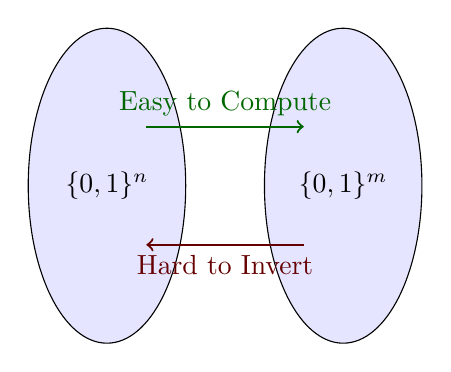
\begin{tikzpicture}
    % ellipse
    \draw[black,fill=blue!10] (0,0) ellipse (1cm and 2cm)
    node at (0,0) {$\{0,1\}^n$};
    \draw[black,fill=blue!10] (3,0) ellipse (1cm and 2cm) 
    node at (3,0) {$\{0,1\}^m$};
    % lines connecting ellipses
    \draw[green!40!black!100, thick, ->] (0.5,0.75) -- (2.5,0.75) node[midway, above] {Easy to Compute};
    \draw[red!40!black!100, thick, ->] (2.5,-0.75) -- (0.5,-0.75) node[midway, below] {Hard to Invert};
\end{tikzpicture}
}


\footnotetext{Typically, the probability is only taken over the random choices of $x$, since we can fix the random coins of the adversary $\mathcal{A}$ that maximize its advantage.}

We note that the function is not necessarily one-to-one. In other words, it is possible that $f(x) = f(x')$ for $x \neq x'$ -- and the adversary is allowed to output any such $x'$.

The above definition is rather delicate. We next describe problems in the slight variants of this definition that are insecure.

\begin{enumerate}
\item What if we require that
    $\Pr_{x \stackrel{\$}{\leftarrow} \binset{n}}[ \mathcal{A}(1^n, f(x)) \in f^{-1}(f(x))] = 0$ instead of being negligible?

This condition is false for every function $f$. An adversary $\mathcal{A}$ that outputs an arbitrarily fixed value $x_0$ succeeds with probability at least $1/2^{n}$, as $x_0 = x$ with at least the same probability.

\item  What if we drop the input $1^n$ to $\mathcal{A}$ in Equation~\ref{eq:owf}?

Consider the function $f(x) = |x|$.  In this case, we have that $m = \log_2 n$, or $n = 2^m$.  Intuitively, $f$ should not be considered a one-way function, because it is easy to invert $f$. Namely, given a value $y$ any $x$ such that $|x| = y$ is such that $x \in f^{-1}(y)$.  However, according to this definition the adversary gets an $m$ bit string as input, and hence is restricted to running in time polynomial in $m$. Since each possible $x$ is of size $n = 2^m$, the adversary doesn't even have enough time to write down the answer!  Thus, according to the flawed definition above, $f$ would be a one-way function.

Providing the attacker with $1^n$ ($n$ repetitions of the $1$ bit) as additional input avoids this issue.  In particular, it allows the attacker to run in time polynomial in $m$ and $n$.
\end{enumerate}

\paragraph{Candidate One-way Functions.}
It is not known whether one-way functions exist. In fact, the existence of one-way functions would imply that $P \neq NP$ (see Exercise~\ref{ex:PNP}). 

However, there are candidates of functions that could be one-way functions, based on the difficulty of certain computational problems. One example is based on the hardness of factoring. Multiplication can be done easily in $O(n^2)$ time, but so far no polynomial time algorithm is known for factoring.
Explicitly, we can define the function $f_1 : P_n \times P_n \rightarrow \mathbb{Z}$ where $P_n$ is the set of all $n$-bit primes as $f_1(p, q) = p \cdot q$.

% One candidate might be to say that given an input $x$, split $x$ into its left and right halves $x_1$ and $x_2$, and then output $x_1 \times x_2$.  However, this is not a one-way function, because with probability $\frac{3}{4}$, $2$ will be a factor of $x_1 \times x_2$, and in general the factors are small often enough that a non-negligible number of the outputs could be factored in polynomial time.

% To improve this, we again split $x$ into $x_1$ and $x_2$, and use $x_1$ and $x_2$ as seeds in order to generate large primes $p$ and $q$, and then output $pq$.  Since $p$ and $q$ are primes, it is hard to factor $pq$, and so it is hard to retrieve $x_1$ and $x_2$.  This function is believed to be one-way.

Another candidate is based on the hardness of the discrete logarithm problem. Given a group $\mathbb{G}$ of prime order $q$ and a generator $g$, the discrete logarithm problem is to find $x$ such that $g^x = y$ for a given $y$. The function $f_2 : \mathbb{Z}_q \rightarrow \mathbb{G}$ defined as $f_2(x) = g^x$ is also believed to be one-way assuming the hardness of the discrete logarithm problem.


\section{Robustness and Brittleness of One-way Functions}
What operations can we perform on one-way functions and still have a one-way function? In this section, we explore the robustness and brittleness of one-way functions and some operations that are safe or unsafe to perform on them.

\subsection{Robustness}
Consider having a one-way function $f$.  Can we use this function $f$ in order to make a more structured one-way function $g$ such that $g(x_0) = y_0$ for some constants $x_0, y_0$, or would this make the function no longer be one-way? 

Intuitively, the answer is yes - we can specifically set $g(x_0) = y_0$, and otherwise have $g(x) = f(x)$.  In this case, the adversary gains the knowledge of how to invert $y_0$, but that will only happen with negligible probability, and so the function is still one-way.

% \begin{theorem}
% Given a one-way function $f : \binset{n} \rightarrow \binset{m}$ and constants $x_0 \in \binset{n}$, $y_0 \in \binset{m}$, $\exists g : \binset{n} \rightarrow \binset{m}$ such that $g(x_0) = y_0$ where $g$ is a one-way function.
% \end{theorem}

In fact, this can be done for an exponential number of $x_0, y_0$ pairs. To illustrate that, consider the following function:
\[
  g(x_1\|x_2) = \left\{ \begin{array}{ll} x_1\|x_2 & : x_1 = 0^{n/2} \\ f(x_1\|x_2) & : \text{otherwise} \end{array} \right.
\]

However, this raises an apparent contradiction - according to this theorem, given a one-way function $f$, we could keep fixing each of its values to $0$, and it would continue to be a one-way function.  If we kept doing this, we would eventually end up with a function which outputs 0 for {\em all} of the possible values of $x$.  How could this still be one-way?\\

The resolution of this apparent paradox is by noticing that a one-way function is only required to be one-way in the limit where $n$ grows very large.  So, no matter how many times we fix the values of $f$ to be 0, we are still only setting a finite number of $x$ values to 0.  However, this will still satisfy the definition of a one-way function - it is just that we will have to use larger and larger values of $n_0$ in order to prove that the probability of breaking the one-way function is negligible.

\subsection{Brittleness}
Given a one-way function $f : \binfunc{n}{n}$, is the function $f^2(x) = f(f(x))$ also a one-way function?  Intuitively, it seems that if it is hard to invert $f(x)$, then it would be just as hard to invert $f(f(x))$. 
% \sanjam{Explain the intuitive reduction that doesn't work.}  
However, this intuition is incorrect and highlights the delicacy when working with cryptographic assumptions and primitives. In particular, assuming one-way functions exists we describe a one-way function $f: \{0,1\}^{n}\times \{0,1\}^{n} \rightarrow \{0,1\}^{2n}$ such that $f^2$ can be efficiently inverted.
Let $g: \{0,1\}^n \rightarrow \{0,1\}^n$ be a one-way function then we set $f$ as follows:
$$f(x_1,x_2) = 0^{n}\|g(x_1)$$
Two observations follow:
\begin{enumerate} 
  \item $f^2$ is not one-way. This follows from the fact that for all inputs $x_1, x_2$ we have that $f^2(x_1,x_2) = 0^{2n}$. This function is clearly not one-way!
  \item $f$ is one-way. This can be argued as follows. Assume that there exists an adversary $\mathcal{A}$ such that $\mu_{\mathcal{A},f}(n) = \Pr_{x \stackrel{\$}{\leftarrow} \binset{n}}[ \mathcal{A}(1^{2n}, f(x)) \in f^{-1}(f(x))]$ is non-negligible. Using such an $\mathcal{A}$ we will describe a construction of adversary $\mathcal{B}$ such that $\allowbreak\mu_{\mathcal{B},g}(n) = \Pr_{x \stackrel{\$}{\leftarrow} \binset{n}}[ \mathcal{B}(1^n, g(x)) \in g^{-1}(g(x))]$ is also non-negligible. This would be a contradiction thus proving our claim.

      \textbf{Description of $\mathcal{B}$}: $\mathcal{B}$ on input $y \in\{0,1\}^n$ outputs the $n$ lower-order bits of  $\mathcal{A}(1^{2n}, 0^{n}\|y)$.

      Observe that if $\mathcal{A}$ successfully inverts $f$ then we have that $\mathcal{B}$ successfully inverts $g$. More formally, we have that:
      $$\mu_{\mathcal{B},g}(n) = \Pr_{x \stackrel{\$}{\leftarrow} \binset{n}}\left[ \mathcal{A}(1^{2n}, 0^n || g(x)) \in \{0,1\}^n || g^{-1}(g(x))\right].$$
      But
      \begin{align*}
      \mu_{\mathcal{A},f}(2n) =& \Pr_{x_1, x_2 \stackrel{\$}{\leftarrow} \binset{2n}}[ \mathcal{A}(1^{2n}, f(x_1, x_2)) \in f^{-1}(f(\tilde x))]\\
      = & \Pr_{x_1 \stackrel{\$}{\leftarrow} \binset{n}}[ \mathcal{A}(1^{2n}, 0^n || g(x_2)) \in \{0,1\}^n || g^{-1}(g(x_2))] \\
      = & \mu_{\mathcal{B},g}(n).
      \end{align*}
      Hence, we have that $\mu_{\mathcal{B},g}(n) = \mu_{\mathcal{A},f}(2n)$ which is non-negligible as long as $\mu_{\mathcal{A},f}(2n)$  is non-negligible.
\end{enumerate}


%\begin{lemma}
%If $f : \binfunc{n}{n}$ is a one-way function, then $g : \binfunc{2n}{2n}$ defined as $g(x) = 0^n \concat f(x_{[1:n]})$ is also one-way.\\
%\end{lemma}
%\proof
%Assume towards contradiction that $g$ is not one-way, and so there is an adversary $A_g$ that inverts $g$ with probability $\mu(2n)$ that is non-negligible.\\
%
%Note that $\mu(2n)$ is also non-negligible with respect to inputs of size $n$.\\

%Then we can define an adversary $A_f$ such that $A_f(y) = (A_g(0^n \concat y))_{[1:n]}$.  Note that $A_g$ breaks $g$ on input $0^n \concat y$ $\implies$ $A_f$ breaks $f$ on input $y$, and so $A_f$ breaks $f$ with at least non-negligible probability $\mu(2n)$.  Contradiction.\\
%
%Thus, $g$ is also one-way.  \qed\\
%
%Now, given a function $f : \binfunc{n}{n}$, we can construct a new one-way function $g : \binfunc{2n}{2n}$.  From $g$, we can construct another one-way function $h : \binfunc{2n}{2n}$ defined by:
%
%$h(x) = \left\{
%\begin{array}{lr}
%  0^{2n} & : x_{[1:n]} = 0^n \\
%  g(x) & : otherwise
%\end{array}
%\right.$

%A generalization of the previous theorem (fixing values in a one-way function) shows that $h$ is also a one-way function.  (In short, we are only fixing the values of $\frac{2^n}{2^{2n}} = \frac{1}{2^n}$ of all of the possible values of $x$.  Since we are only fixing a negligible fraction of the possible values of $x$, the same proof with slight modifications still applies.)\\
%
%So, $h$ is a one-way function.  However, $h^2(x) = h(h(x)) = 0^{2n}$, and so $h^2$ is clearly not a one-way function.  Thus, composing one-way functions is not guaranteed to give another one-way function. \qed


